\section{Precalentamiento}

\begin{itemize}
    \item Para el tercer ejercicio Python discrimina los datos enteros con los de tipo string.
    \item Para el último ejercicio Python reconoce los valores booleanos por separado, en este caso bool('A') y bool('g' in a).
\end{itemize} 

\begin{figure}[h]
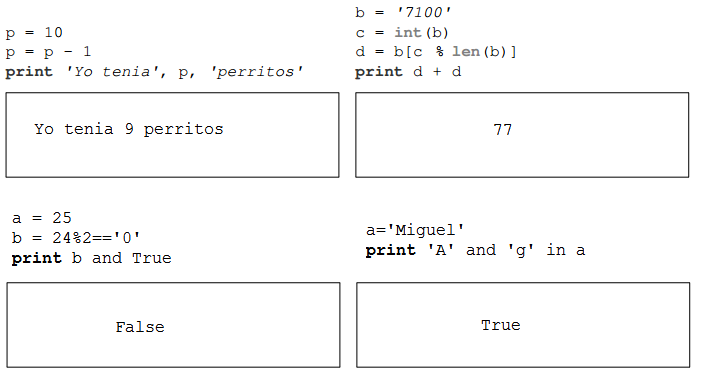
\includegraphics{imagenes/pauta1.png}
\end{figure}
